\documentclass[11pt,twoside,a4paper]{article}
\usepackage{amsmath}
\usepackage{amssymb}
\usepackage{geometry}
\usepackage{multicol}% multi colomn
\usepackage{graphicx}
\usepackage{float}
\geometry{a4paper,left=2cm,right=2cm,top=1cm,bottom=2cm}
\DeclareMathSizes{12}{20}{14}{10}
\begin{document}
\title{Ex7 186 Fall}
\author{Assignment group 10}
\date{}
\maketitle

\section{Ex7.4}
\begin{figure}[H]
    \centering
    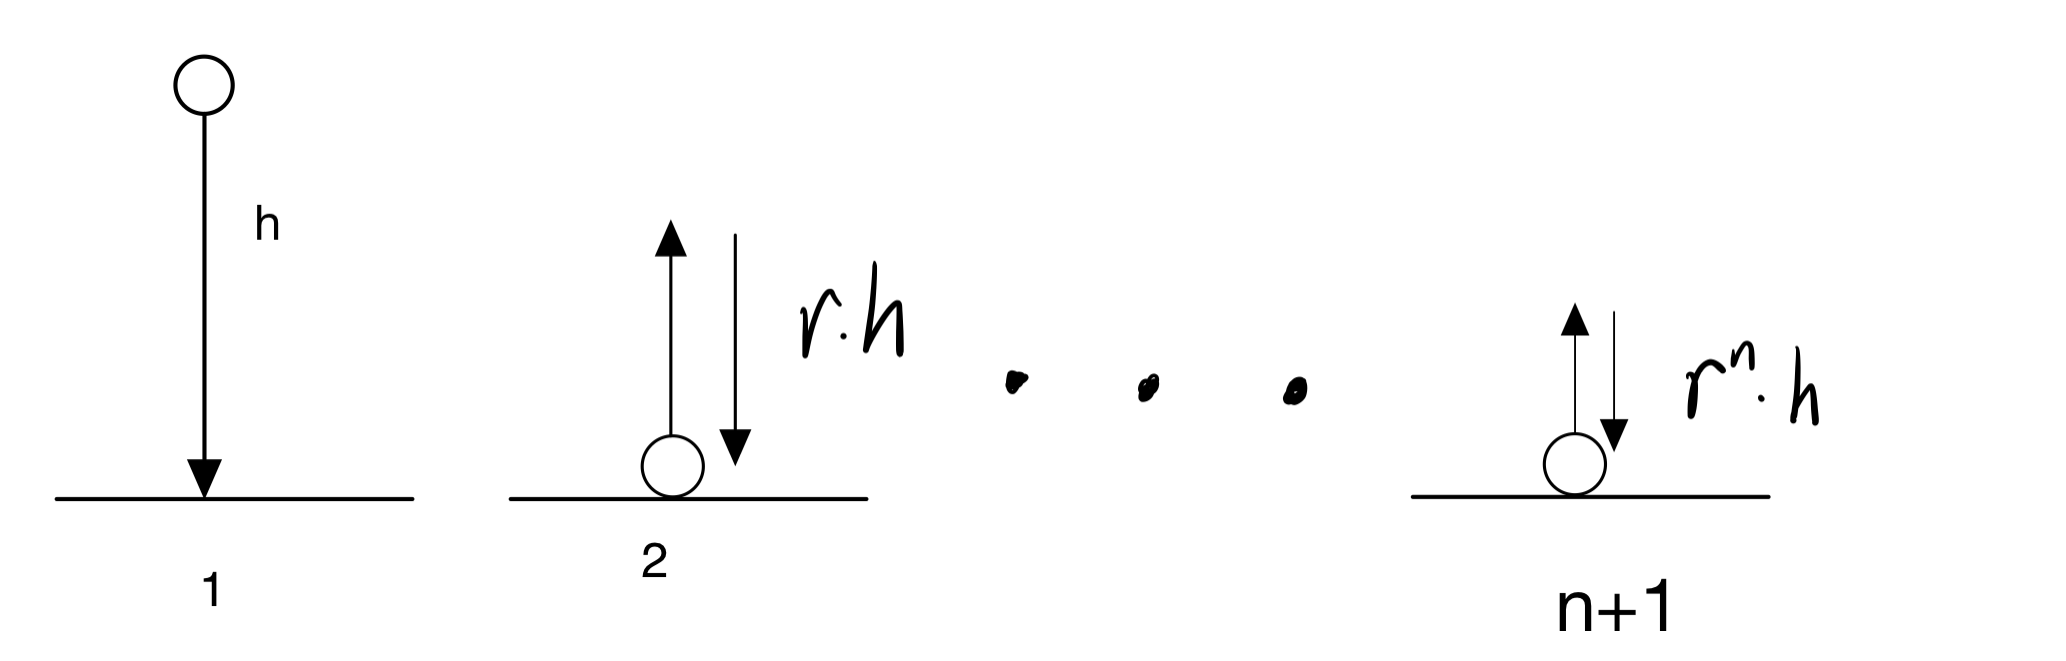
\includegraphics[scale=0.5]{Ex7.4.png}
    \caption{Figure 7.4}
    \end{figure}
The distance can be assessed through the image above (figure Ex7.4).
\par 
The first process : $h$
\par 
The second process : $2r\cdot h$
\par 
$. . .$
\par 
The $n$th process : $2r^{n-1}\cdot h$
\newline
Except for the first process is one-way, other process are all double-way
Thus, the total distance :
\begin{equation}
    \begin{aligned}
        D&=2(\sum_{n = 1}^{\infty} r^{n-1} \cdot h)-h\\
        &=\frac{2h}{1-r}-h
    \end{aligned}
    \end{equation}

\section{Ex7.5}
We can know from the question that 
$$\displaystyle \sum \frac{1}{n}= \sum _{n\in X} \frac{1}{n} +\sum _{n \in \mathbb{N}^* \backslash X} \frac{1}{n}$$
Because 
\begin{equation}
    \begin{aligned}
        \displaystyle \sum _{n \in \mathbb{N}^* \backslash X} \frac{1}{n} &=
        \frac{1}{9}+\frac{1}{81}+\dots+\frac{1}{9^k}+\dots\\
        &=\frac{1}{9}\sum \frac{1}{n}
    \end{aligned}
    \end{equation}
So, $\displaystyle \sum _{n \in \mathbb{N}^* \backslash X} \frac{1}{n}$ diverges.
\newline
Then, we can find that $\displaystyle\sum _{n\in X} \frac{1}{n}=\frac{8}{9}\sum \frac{1}{n}$
So, $\displaystyle \sum _{n \in X} \frac{1}{n}$ also diverges.


\section{Ex7.6}
\begin{figure}[H]
    \centering
    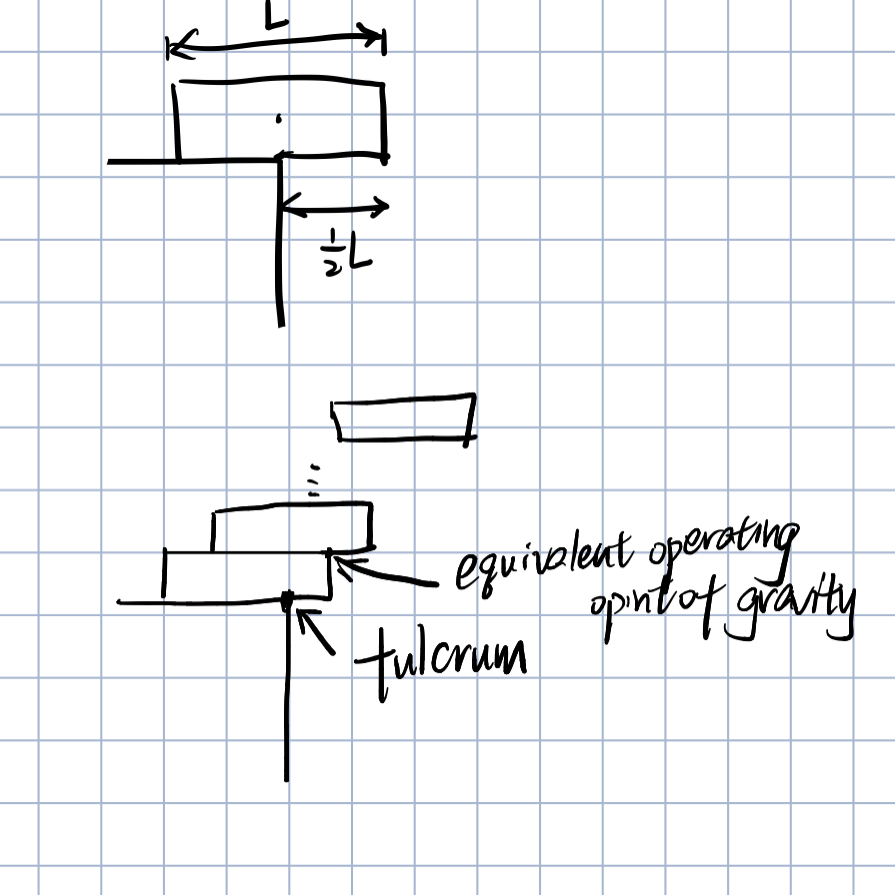
\includegraphics[scale=0.5]{Ex7.6.1.png}
    \caption{Figure 7.6.1}
    \end{figure}
We can model the question(figure 7.6.1). When there are $n+1$ bricks,
 assume that the mass of each brick is $m$, the acceleration 
 of gravity is $g$, the length of the lever is $L$ and the 
 distance between the middlepoint and the right end is 
 $l_{n+1}$. We can then simplify it into a lever (show in figure 7.6.2).
\begin{figure}[H]
    \centering
    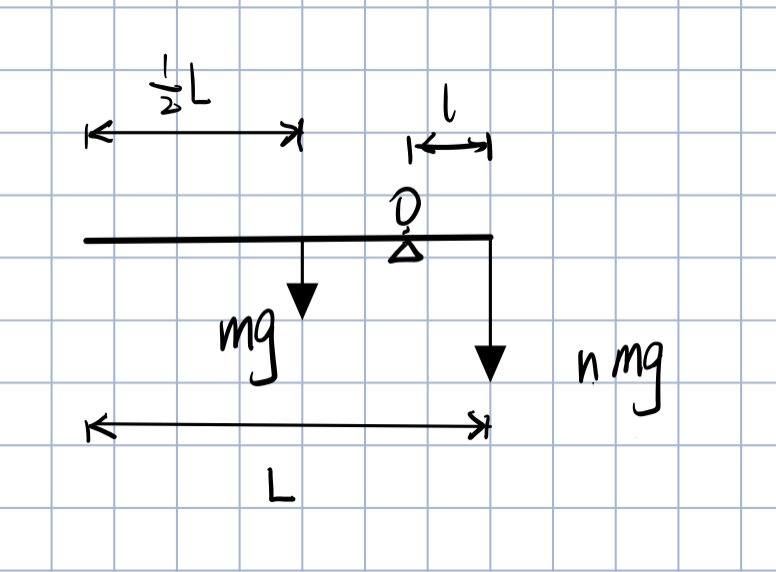
\includegraphics[scale=0.5]{Ex7.6.2.png}
    \caption{Figure 7.6.2}
    \end{figure}
    According to lever principle, we can know that 
\begin{equation}
    \begin{aligned}
        mg(\frac{L}{2}-l_{n+1})&=nmgl_{n+1}\\
        \frac{1}{2}mgL-mgl_{n+1}&=nmgl_{n+1}\\
        l_{n+1}&=\frac{L}{2(n+1)}\\
        l_{n+1}&=\frac{L}{2}\cdot\frac{1}{n+1}
    \end{aligned}
    \end{equation}
So we can know $\sum_{n = 1}^{\infty}l_{n+1} $ diverges. Thus, 
the tower can extend to infinite far.

\section{Ex7.7}
\subsection{7.7.1}
\begin{equation}
    \begin{aligned}
        \sum_{n = 1}^{\infty}  \frac{2^{2n}\cdot 3^{3n}}{5^{3n}}&=
        \sum_{n = 1}^{\infty} \frac{4^n 27^n}{125^n}\\
        &=(\frac{108}{125})^n\\
        &=\frac{108}{17}
    \end{aligned}
    \end{equation}
    So, we can know the $\displaystyle\sum_{n = 1}^{\infty}  \frac{2^{2n}\cdot 3^{3n}}{5^{3n}}$
    converges.
\subsection{7.7.2}
Because we know when $n>3$, $n^2-3n+1>0$
Thus, we can know:
\begin{equation}
    \begin{aligned}
        a_{n}:=\sum_{n = 1}^{\infty}  \frac{n+4}{n^2-3n+1}&=
        \sum_{n = 1}^{3}  \frac{n+4}{n^2-3n+1}+
        \sum_{n = 4}^{\infty}  \frac{n+4}{n^2-3n+1}\\
        &>\sum_{n = 1}^{3}  \frac{n+4}{n^2-3n+1}+
        \sum_{n = 4}^{\infty}  \frac{n+4}{n^2+16n+16}\\
        &=\sum_{n = 1}^{3}  \frac{n+4}{n^2-3n+1}+
        \sum_{n = 4}^{\infty}  \frac{1}{n+4}=:b_{n}
    \end{aligned}
    \end{equation}
Because $\displaystyle \sum_{n = 4}^{\infty}  \frac{1}{n+4}$ diverges, so $b_{n}$ diverges.
\newline
Thus $\displaystyle a_{n}=\sum_{n = 1}^{\infty}  \frac{n+4}{n^2-3n+1}$ diverges
as $0<b_{n}<a_{n}$.

\subsection{7.7.3}
Let $\displaystyle a_{n}:=\frac{n^4}{3^n}$. We will use deduction to 
prove that when $n \ge 32$, $n^4<2^n$.
\newline
Firstly, when $n=32$, $(32)^4=2^{20}<2^{32}$
\newline
Secondly, assume that when $n=k$,$n \in \mathbb{N}^*,k\ge 32$
, we also have $2^k>k^4$.
\newline
So, when $n=k+1$, because
$$\frac{(k+1)^4}{k^4}=(\frac{k+1}{k})^4<(\frac{33}{32})^4<2$$
Thus, 
$$2^{k+1}=2\cdot 2^{k}>2\cdot k^n >(k+1)^4$$
So, we have proved that when $n \ge 32$, $n^4<2^n$.
\newline
We get 
$$\sum_{n = 1}^{\infty} a_{n} =\sum_{n = 1}^{32} a_{n} 
+\sum_{n = 33}^{\infty}\frac{n^4}{3^n}
<\sum_{n = 1}^{32}a_{n}+
\sum_{n = 33}^{\infty} (\frac{2}{3})^n:=b_{n} $$
\newline
Because we know that $\displaystyle \sum_{n = 33}^{\infty} (\frac{2}{3})^n$
converges.
So, $b_{n}$ converges. Thus $a_{n}$ converges as $0<a_{n}<b_{n}$,

\subsection{7.7.4}
Let $\displaystyle a_{n}:=\frac{2^n}{n!}$, Then, 
$$\displaystyle 
\lim_{x \to \infty} \frac{a_{n+1}}{a_{n}}
=\lim_{x \to \infty}\frac{\frac{2^{n+1}}{(n+1)!}}{\frac{2^n}{n!}} 
=\lim_{x \to \infty} \frac{2}{n+1}=0$$
Thus,$\displaystyle a_{n}=\frac{2^n}{n!}$ converges.

\subsection{7.7.5}
Let $\displaystyle a_{n}:=\frac{2^n}{n^n}$. Then,
$$\displaystyle \lim_{x \to \infty} \frac{a_{n+1}}{a_{n}}
=\lim_{x \to \infty} \frac{2n^n}{(n+1)^(n+1)}
=\lim_{x \to \infty} 2\cdot(\frac{n}{n+1})^n \cdot (\frac{1}{n+1})
=0 $$
Thus, $\displaystyle a_{n}=\frac{2^n}{n^n}$ converges.

\subsection{7.7.6}
We can know from 
$\displaystyle \sum_{n = 1}^{\infty} \frac{n}{10n^3-100} $
that when $n>4$, $\displaystyle \sum_{n = 1}^{\infty} \frac{n}{10n^3-100}>0 $
\newline
And then, we will prove that when $n>4$, $\displaystyle \frac{n}{10n^3-100}>0 $
strictly decreases.
\par
Proof:\newline
For $\forall n>4$ , 
\begin{equation}
    \begin{aligned}
        \frac{n+1}{10(n+1)^3-100}-\frac{n}{10n^3-100}
        &=\frac{1}{10}(\frac{n+1}{(n+1)^3-10}-\frac{1}{10}(\frac{n}{n^3-10}) \\
        &=\frac{1}{10}\cdot\frac{-2n^3-3n^2-n-10}{[(n+1)^3-10](n^3-10)}<0
    \end{aligned}
    \end{equation}
Thus, $\displaystyle \frac{n}{10n^3-100}>0 $ strictly decreases.\newline
Then, we will prove $a_{n}:=\sum_{n = 1}^{k}\displaystyle \frac{n}{10n^3-100}$ is Cauchy squence.
\par
Proof:\newline
For all $n>4$ and fixed $p$, 
\begin{equation}
    \begin{aligned}
        \sum_{n = 1}^{k+p} \frac{n}{10n^3-100}-\sum_{n = 1}^{k} \frac{n}{10n^3-100}
        =\sum_{n = k+1}^{k+p} \frac{n}{10n^3-100}
    \end{aligned}
    \end{equation}

Because 
\begin{equation}
    \begin{aligned}
        \left|\sum_{n = k+1}^{k+p} \frac{n}{10n^3-100}-\sum_{n = k+2}^{k+p+1} \frac{n}{10n^3-100}\right|
        &=\frac{k+p+1}{10(k+p+1)^3-100}-\frac{k+1}{10(k+1)^3-100} \\
        &<\frac{p}{10(k+1)^3-100}
    \end{aligned}
    \end{equation}
    We can know that $\displaystyle \lim_{k \to \infty} \frac{p}{10(k+1)^3-100} =0$. So 
    $\forall \varepsilon>0,\exists k \in \mathbb{N}^*$, there exists $\varepsilon$ that satisfies
    $$\left|\sum_{n = 1}^{k+p} \frac{n}{10n^3-100}-\sum_{n = 1}^{k} \frac{n}{10n^3-100}\right|<\varepsilon$$
    We have prove $a_{n}:=\sum_{n = 1}^{k} \displaystyle \frac{n}{10n^3-100}$ is Cauchy squence.
    And then we can know $\displaystyle \sum_{n = 1}^{\infty} \frac{n}{10n^3-100} $ converges.
\end{document}
